\documentclass[a4paper, 12pt, final, garamond]{book}
\usepackage{cours-preambule}

\raggedbottom

\makeatletter
\renewcommand{\@chapapp}{Travaux pratiques -- TP}
\makeatother

\let\SavedIndent\indent
\protected\def\indent{%
  \begingroup
    \parindent=\the\parindent
    \SavedIndent
  \endgroup
}
\setlength{\parindent}{0pt}

\begin{document}
\setcounter{chapter}{0}

\chapter{D\'etermination de focales de lentilles}

\section{Objectifs}

\begin{itemize}
    \item	Réaliser des alignements sur un banc optique~;
    \item Reconnaître rapidement une lentille convergente et une lentille
        divergente~;
    \item Déterminer une distance focale par différentes méthodes.
\end{itemize}

\section{S'approprier}

Trois méthodes sont possibles pour la détermination expérimentale de la distance
focale d'une lentille convergente.

\subsection{Méthode de Bessel}
	
La méthode de Bessel utilise le montage ci-dessous où $D$, la distance
objet-écran, est fixée, avec $D>4f'$.

\centers{
	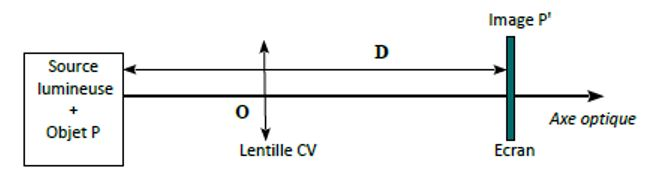
\includegraphics[width=\linewidth]{schema1}
}

La méthode de Bessel pour déterminer la distance focale $f'$ consiste donc à
imposer une distance $D$ entre un objet et un écran et à rechercher les deux
positions de la lentille $L$ qui donnent une image nette de l'objet sur l'écran
$E$. En mesurant les deux distances $D$ et $d$ (distance entre les deux
positions de la lentille pour lesquelles on obtient une image nette), on peut
calculer la valeur de la distance focale image $f'$ de la lentille.

\subsection{Méthode de Silbermann}

La méthode de Silberman est le cas particulier de la méthode de Bessel pour
lequel $D=4f'$.

\subsection{Utilisation de la relation de conjugaison}

Cette méthode consiste à utiliser une régression linéaire permettant de vérifier
la relation de conjugaison~: 

\centers{$\dfrac{1}{\obar{OA'}}-\dfrac{1}{\obar{OA}} = \dfrac{1}{f'}$}

\section{Analyser}

\subsection{Méthode de Bessel}

\begin{minipage}{0.49\linewidth}
    A l'aide d'une lentille mince convergente $(L)$ de distance focale image
    $f'$, on veut former l'image d'un objet réel sur un écran situé à une
    distance $D$ de l'objet. En déplaçant la lentille, on trouve une ou deux
    positions $O_1$ et $O_2$ qui donnent une image nette sur l'écran (cf. figure
    ci-contre).

\end{minipage}
\begin{minipage}{0.49\linewidth} 
  \begin{center}
    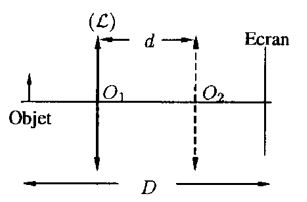
\includegraphics[width=0.9\textwidth]{schema2}
  \end{center}
\end{minipage} 

\begin{enumerate}
    \item Déterminer dans ce cas, les deux expressions des positions
        correspondantes de la lentille notées $x_1=\obar{O_1A}$ et
        $x_2=\obar{O_2A}$ en fonction de $D$ et $f'$ et vérifier que
        celles-ci n'existent que si $D>4f'$.
    \item Exprimer $d=\obar{O_1O_2}$ , puis montrer qu'alors
        \centers{$f'=\dfrac{D^2-d^2}{4D}$}
    \item Déterminer un protocole expérimental permettant la mesure d'une
        distance focale par cette méthode.
\end{enumerate}

\subsection{Méthode de Silbermann}

\begin{enumerate}
    \item Montrer qu'il existe un cas particulier intéressant où $x_1=x_2$. 
    \item En déduire la nouvelle expression de $f'$ dans ce cas. 
    \item Déterminer un protocole expérimental permettant d'utiliser cette
        deuxième méthode.
\end{enumerate}

\subsection{Méthode utilisant la relation de conjugaison}

Déterminer un protocole expérimental permettant d'utiliser cette troisième
méthode. Vous l'expliciterez clairement et le proposerez au professeur avant
mise en application. 

\section{Réaliser}

\subsection{Matériel disponible}

\begin{itemize}
    \item Lentilles convergentes et divergentes (en dioptries, $\delta$)~: -10~;
        -3~; -2~; -1~; 1~; 2~; 3~; 8~; 10.
    \item Lampe spectrale
    \item Écran dépoli
    \item Banc d'optique et supports
    \item Support magnétique constitué des lettres $F$ et de la mini-règle 
    \item Écran 
    \item Réglet
\end{itemize}

\subsection{Reconnaissance rapide convergente ou divergente}
	
\begin{instruc}{Attention}
    Afin de se protéger de la lumière émise par la lampe, insérer un écran
    dépoli entre la lampe et l'objet.
\end{instruc}

Avec les lentilles disponibles, vérifier expérimentalement les critères suivants
après les avoir expliqués de manière théorique à l'aide de tracés de rayons~:

\begin{enumerate}
    \item \textbf{Observation directe}~: Les lentilles convergentes sont des
        lentilles à bords minces, les lentilles divergentes sont à bords épais.
    \item \textbf{Effet loupe}~: Une lentille convergente donne d'un objet placé
        à faible distance une image virtuelle, droite et agrandie.
    \item \textbf{Effet anti-loupe}~: Une lentille divergente donne d'un objet
        réel proche ou éloigné une image virtuelle, droite et réduite.
    \item \textbf{Déplacement transversal}~: Lorsqu'on déplace transversalement
        une lentille convergente devant un objet placé à faible distance, son
        image se déplace dans le sens inverse de celui de la lentille.  Dans le
        cas d'une lentille divergente, le sens du déplacement est identique.
\end{enumerate}

\subsection{Projection sur un écran avec une lentille convergente}

\begin{enumerate}
    \item Réaliser un alignement sur le banc d'optique permettant de projeter
        l'image d'un objet sur un écran à l'aide d'une lentille convergente.
    \item Pour une position de la lentille donnée, déterminer le grandissement
        $\gamma=\dfrac{\obar{A'B'}}{\obar{AB}}$ et vérifier la relation~:

        \centers{$\gamma=\dfrac{\obar{OA'}}{\obar{OA}}$}

        en mesurant $\obar{OA'}$ et $\obar{OA}$ à l'aide d'un réglet.
\end{enumerate}

\subsection{Mesure précise de la distance focale d'une lentille convergente}

Mettre en œuvre les trois méthodes proposées dans les parties analyser et
s'approprier pour déterminer la distance focale de la lentille convergente notée
($+10$). Comparer les résultats obtenus par les différentes méthodes. Vous
calculerez dans chaque cas l'écart relatif par rapport à la valeur théorique. 


\section{Valider et conclure}

Déterminer l'incertitude-type sur la détermination de la distance focale $f'$
obtenue dans le cas de la méthode de Bessel. On évaluera dans un premier temps
l'incertitude de type B sur la détermination de $D$ et $d$ puis on en déduira
l'incertitude-type sur $f'$ par méthode de Monte-Carlo. (voir Fiche pratique~:
on adaptera le programme exemple fourni dans la fiche)

% \vspace{3cm}
% \begin{programme}{}
% 
% \vspace{1cm}
% \begin{itemize}
% \item Former une image. 
% \item Modéliser    expérimentalement    à    l'aide    de 
% plusieurs     lentilles     un     dispositif     optique 
% d'utilisation courante. 
% \item Éclairer un objet de manière adaptée. 
% \item Optimiser   la   qualité   d'une   image   (alignement, 
% limitation des aberrationsÉ). 
% \end{itemize}
% \end{programme}

\end{document}

